\chapter{Methods}

Nine samples of mud- and siltstones were collected near the village
of Vorderthal along the tectonic contact between the SMB and the Helvetic 
nappe~(\cref{fig:study_area}). 
These were the primary samples for this study. In addition, one flysch sample from the Helvetic nappe
(marked in blue on the map in \cref{fig:study_area}), and one \OSM sample
from near Leimbach outside the main study area (orange dot in the
overview inset in \cref{fig:study_area}) were collected
as reference samples representing a marine and terrestrial
facies, respectively. The sample locations and corresponding samples
were designated ``JWL $x$'', where $x$ is an increasing number.

Concentrations of the elements \acro{Sr}, \acro{Ba}, \acro{Cl}, 
\acro{Br}, and \acro{S} as well as \TOC were determined using \XRF, \ICPMS
and the TOC-only mode of isotope-ratio mass spectrometry (\acro{IRMS}).
\XRF should be able to determine all target elements except carbon~\parencite{ichikawa_solid_2023}, \ICPMS
can measure trace metals and, with appropriate digestion methods, halogens~\parencite{he_rapid_2018}. 
IRMS combustion analysis is specific to \TOC~\parencite{irms}.
Using several methods for each element enables cross-validation 
of the results, and helps identify the most suitable method for individual elements.

The computed concentration ratios for Sr/Ba and S/TOC were compared against published classification thresholds
by \textcite{berner-raiswell-1983,wei-2020}. An approximate best fit threshold was computed
using the Receiver Operating Characteristic (ROC) curve approach \parencite{fawcett-roc-2006}.
In all cases, samples are classified as marine when their trace-element ratio exceeds a specified threshold.
The ROC algorithm tests which of the computed ratios in our dataset best reproduces the classification 
from the geological map.
Because of the mathematical properties of ROC curves, selecting the best fit threshold
using Youden's J statistic yields an approximation that minimizes classification errors \parencite{youden-index-2019}.

\section{Rock powder preparation}

All measurement methods use fine rock powder as the starting material. 
The samples were therefore processed following a protocol adapted from \textcite{ichikawa_solid_2023}:
\begin{enumerate}
    \item Samples were first dried at 40\degree C for at least one week.
    
    \item Approximately 60\,g of the samples were crushed and then milled for 4 minutes in a
    tungsten carbide vessel on a vibrating mill. 
    Milling was extended to 8 minutes when necessary to achieve sufficiently fine powder.
    
    \item The powders were dried at $100 \pm 5$\degree C for at least 24\,h and
    cooled in a desiccator, and then stored in closed but not sealed containers.
\end{enumerate}


\section{X-Ray Fluorescence (\XRF)}

\XRF measures the characteristic fluorescence of atoms caused by irradiation with X-rays.
Reliable measurements require the irradiated sample to be homogenous across
the entire analysed volume. Homogeneity is achieved by using
fine rock powder as the sample. This powder can either be pressed into a pellet
together with a binding agent, or it can be fused with a borate-based flux to
produce glass beads~\parencite{ichikawa_solid_2023}.
The high temperatures required to melt the borate flux cause volatiles like
halogens and sulphur to evaporate.
To preserve all volatiles, for this study we used powder pellets. 

To obtain consistent, reproducible results, the grain sizes in samples should be smaller than the analytical 
depth and the thickness of the pellet should exceed the escape depth~\parencite{ichikawa_solid_2023}.
The escape depth is always smaller than the analytical depth, which can be obtained from
standard tables~(cf.~\cref{tab:xrf-analytical-depth}).
A powder pellet suitable for the XRF unit at \ETH is a disc
approximately 4\,cm in diameter and 3-4\,mm thick (\cref{fig:xrf-pellets}). The 4\,mm thickness of the pellets
is sufficient for our target elements.

% For accurate and repeatable measurements \textcite{ichikawa_solid_2023} suggested
% adjusting the powder grain size and the pellet's surface smoothness to the elements of
% interest.
% The \emph{escape depth} or \emph{analytical depth} of fluorescent X-rays depends on their wavelength and the 
% average density of the material of the pellet. 
% \emph{Escape depth} refers to the maximum depth from within the pellet that fluorescent radiation of
% a specific wavelength can still escape instead of being absorbed by heavy atoms in the sample.
% \emph{Analytical depth} refers to how deeply the irradiating X-rays can penetrate the sample.
% Both of these are governed by the properties of the sample material and the elements we want to measure.

% How far X-rays can penetrate a material
% is governed by the Lambert-Beer law

% \begin{equation}\label{eq:lambert}
%     I = I_0 \exp(-\mu_\lambda \cdot \rho \cdot d)
% \end{equation}

% where $I$ is the intensity of the X-rays of initial intensity $I_0$ after penetrating a material
% to depth $d$ in a sample of average density $\rho$ 
% with a mass absorption coefficient of $\mu_\lambda$. Rearranging \cref{eq:lambert} and setting
% $I=I_0/2$ yields a formula for the \emph{half-thickness}, the depth at which the initial intensity 
% has halved:

% \begin{equation}
%     \frac{I_0}{2} = I_0 \exp(-\mu_\lambda \cdot \rho \cdot d) \Leftrightarrow d_{0.5} = \frac{\ln 2}{\mu_\lambda\cdot\rho}
% \end{equation}

% \textcite{ichikawa_solid_2023} estimated the escape depth to be four times the half-thickness.
% For most analyses it is sufficient to estimate the analytical depth. Therefore, using tabled values for
% the mass absorption coefficient and average densities for common rock types is acceptable (cf.~\cref{tab:xrf-analytical-depth}).


\begin{figure}[b]
  \nopagebreak
  % Left side: The Figure
  \begin{minipage}[b]{0.45\textwidth}
    \vfill
    \centering
    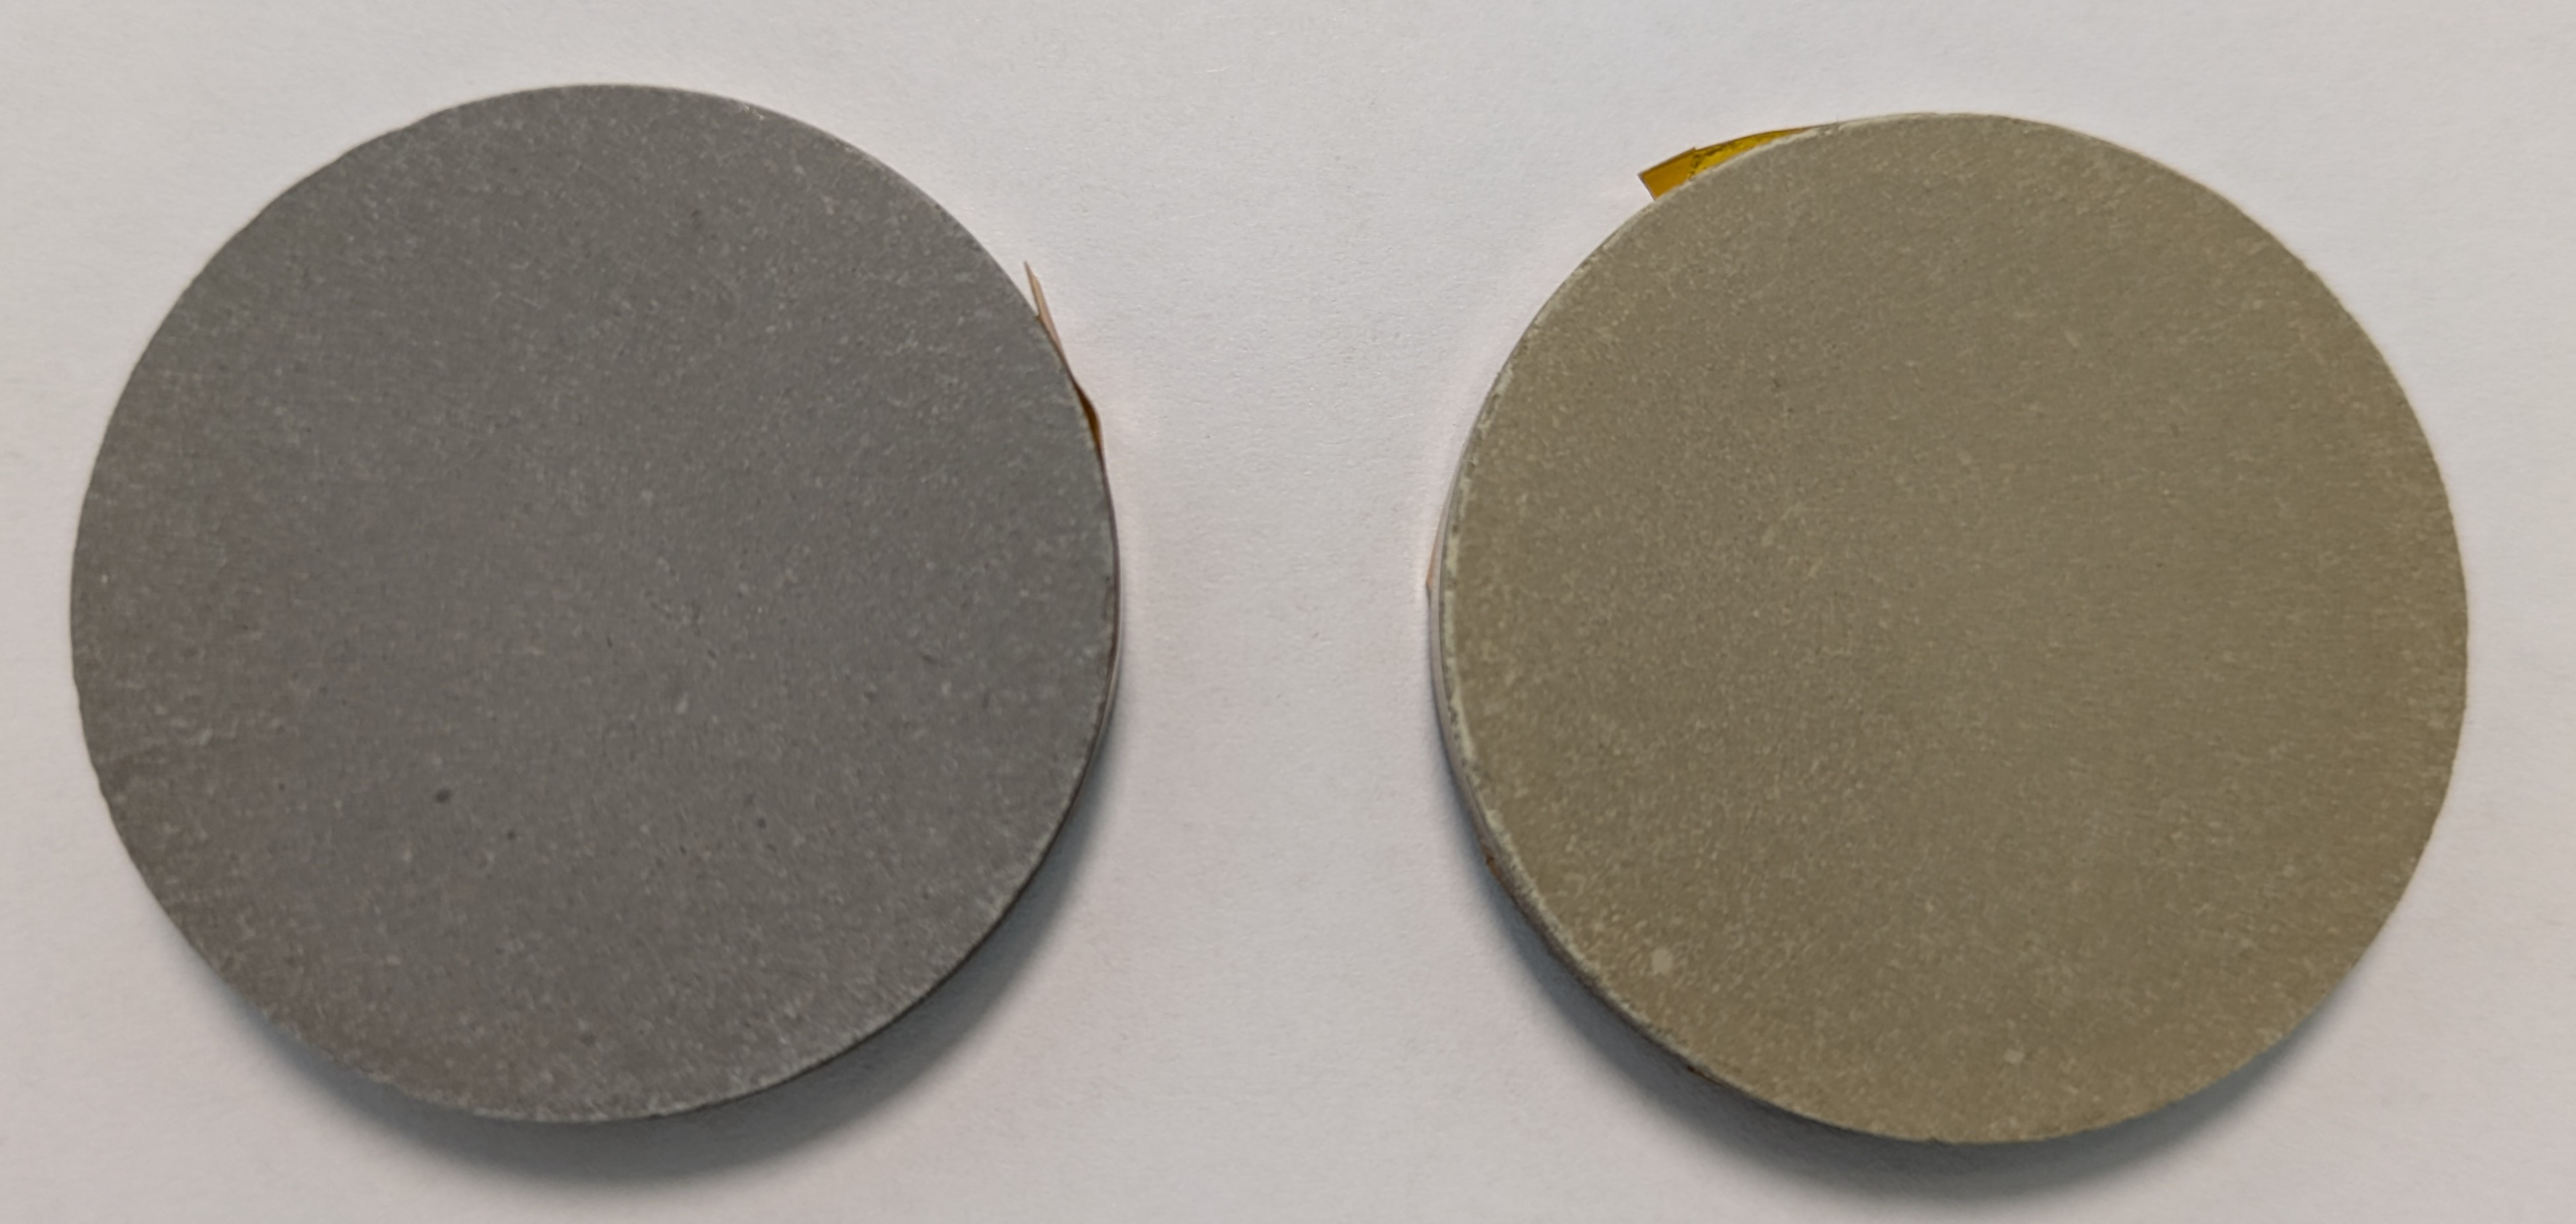
\includegraphics[width=0.95\textwidth]{img/xrf_pellets.jpg}
    \captionsetup{width=0.95\linewidth}
    \caption{Pellets for rock samples JWL 1 and JWL 2.}
    \label{fig:xrf-pellets}
  \end{minipage}
  \hfill % Adds horizontal space between the minipages
  % Right side: The Table
  \begin{minipage}[b]{0.48\textwidth}
    \centering
    \captionsetup{width=0.95\linewidth}
    \captionof{table}{Analytical depths for elements of interest, estimated with Bruker's online
    ``XRF Check'' calculator \parencite{bruker-xrf-check}.}
    \label{tab:xrf-analytical-depth}
    \begin{tabular}[b]{ll}
        \toprule
        \textbf{Element} & \textbf{Analytical depth [$\mu$m]} \\\midrule
        Ba &  4500 \\
        Br & 427\\
        Cl & 5.34 \\
        S & 3.77 \\
        Sr & 660 \\        
        \bottomrule
    \end{tabular}
  \end{minipage}
\end{figure}

\subsection{Sample preparation}
 
Because we did not have access to a means to control the grain size of the powders we produced, 
we used a standard protocol used for the preparation of powder \XRF pellets at \ETH:

\begin{enumerate}
    \item Sample powder and binding agent were mixed at a mass ratio of 8:2 for
    a total of 10\,g. 
    \item The mixture was homogenized in 
    a shaker for 4 minutes; in few cases 8 minutes were required.
    \item The mixture was pressed into pellets of 40\,mm diameter with a stepwise pressure increase  
    of 100, 200, 300, 400, 450\,bar, holding each pressure for 20 seconds without releasing pressure
    between steps.
\end{enumerate}

Some samples did not form stable pellets at the 8:2 ratio. In those cases powder:binder
ratios of 7:3 and 6:4 were tried and yielded stable pellets.
Two pellets were produced and analysed for each rock sample, 

\subsection{Measurements}

All samples were analysed using a Bruker Tiger S8 WDXRF unit\footnote{\url{https://www.bruker.com/en/products-and-solutions/elemental-analyzers/xrf-spectrometers/s8-tiger.html}}
(20kV-60kV) with a Rhodium anode to determine
concentrations of \acro{Cl}, \acro{Br}, \acro{Sr}, \acro{Ba} and \acro{S}.
Because the instrument was not yet calibrated with certified reference materials
and certified rock standards for the rocks we analysed were not available, we used the
fundamental parameter method~\parencite{ichikawa_solid_2023}.
Therefore, the accuracy of the results is likely less than it could be. 

For each measurement, the analytical software reports all elements above their respective detection limits.
It also provides the \emph{Compton ratio} as an indication
of how reproducible, and thus how representative of the sample, that measurement is estimated to be.

\section{ICP mass spectrometry}

\ICPMS requires samples to be in liquid form so they can be aerosolized 
and injected into the plasma chamber where they are vaporized and ionized 
before entering the mass spectrometer.
For rock samples, digestion with \acronym{HF}{hydrofluoric acid} is commonly used 
to produce the required solution for trace metal analysis~\parencite{hu-digestion-2014}. 
\textcite{he_rapid_2018} also applied this
method to extract halogens. In addition, they proposed \acronym{\ambif}{ammonium bifluoride}
as a solid flux that improves halogen retention and reduces the impact of 
aggressive acids on the instrument~\parencite{he_determination_2019}.

We used \acro{HF} digestion to obtain concentrations of all elements
that remain stable during the digestion process. Because halogens \emph{are} volatile and
leave the resulting slurry, 
we also used \ambif\ digestion to accurately measure \acro{Cl} and \acro{Br}, following the
procedure described by \textcite{he_determination_2019} as closely as possible.

For both digestion methods, we measured the two common 
rock standards BCR-2 and BHVO-2 for quality control~\parencite{bcr2, bhvo2}.
Additionally, for the digestion with \acro{\ambif} we prepared several
reagent blanks containing only \acro{\ambif} to quantify and correct for 
impurities in the reagent.

\subsection{Sample preparation}

\subsubsection{\ambif\ digestion}
\begin{enumerate}
\item 100\,mg of sample were weighed into a Teflon vial.
\item 400\,mg of \ambif\ were added into the vial.
\item The mixture was heated to 200-220\degree C for 2\,h in closed, but not sealed vials.
After cooling, this should result in a solid digestion cake.
\item This residue was washed and partially dissolved with 5\,ml 5\% NH$_3$ solution.
\item The resulting mix of slurry and solution was centrifuged for 10 minutes.
\item The supernatant was taken as the solution for \ICPMS.
\end{enumerate}

\textcite{he_determination_2019} did not provide enough detail how to move from step 3 to step 6. 
They only state ``The digestion cake was diluted by 5\% v/v NH$_4$OH
solution to 25 g after cooling.''~\parencite[p. 8110]{he_determination_2019}.
This presumes that the halogens remain in the digestion cake, and not in the atmosphere of the vial.
The vial volume (7\,ml) makes dilution to 25\,g total mass impossible. 
Consequently, the cake would have to be transferred to a 
larger vessel. This can lead to loss of material, and thus measurement uncertainty.

Because \ambif\ digestion is an untested technique at \ETH, we prepared three vials each for the \OSM and flysch
samples to quantify the measurement variability for identical rock samples.

% \begin{figure}
%     \centering
%     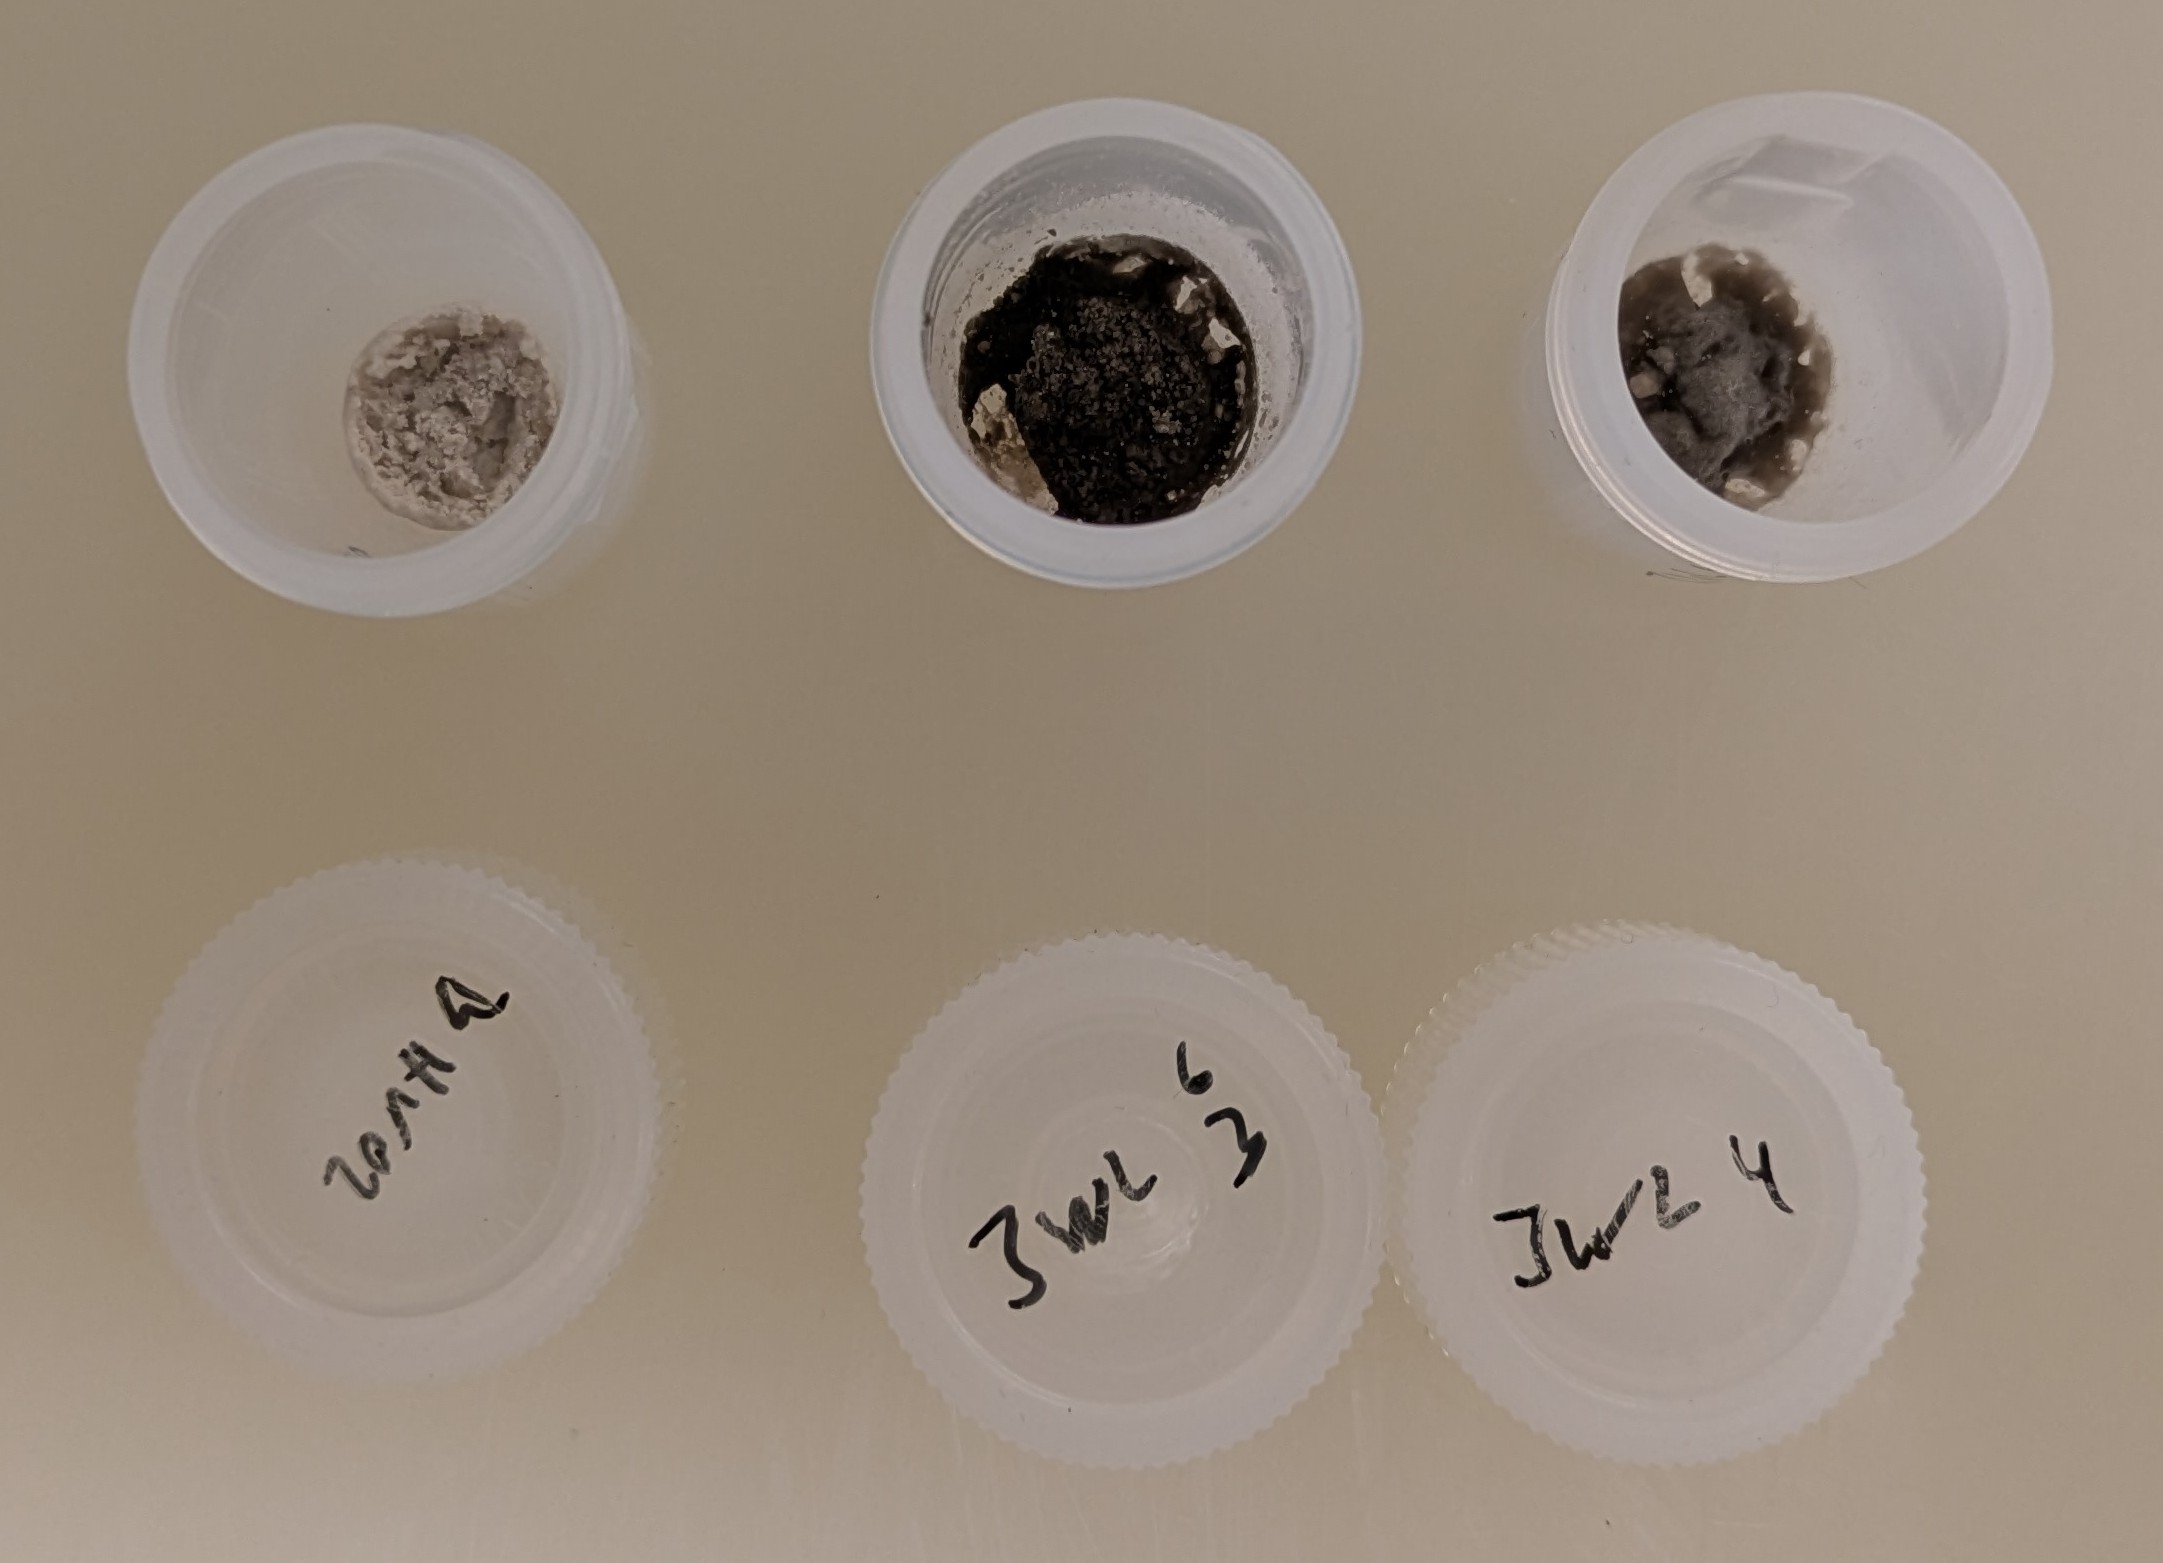
\includegraphics[width=0.45\textwidth]{img/NH4_samples.jpg}
%     \caption{Photograph of some sample vials with the digestion cake after step 3. }
%     \label{fig:NH4-samples}
% \end{figure}

\subsubsection{HF digestion}

The protocol for \acro{HF} digestion is similar to the one for \ambif:

\begin{enumerate}
\item 5\,mg of sample were weighed into a Teflon vial.
\item A mixture of concentrated \acro{HF} and concentrated nitric acid (\acro{HNO$_3$}) 
    was added to the sample vial.
\item The mixture was heated on a hotplate to 200-220\degree C for two days.
\item The resulting solution was diluted with 2\% nitric acid and directly used for \ICPMS.
\end{enumerate}

\subsection{Measurements}

Both sets of samples were measured following the standard procedure at \ETH.
Blank solutions were measured first to define the instrumental background.
Then internal reference standards were measured to allow drift correction of later measurements.
The rock samples were measured in batches of five, and after each batch
the reference standards were measured again to detect instrument drift. 


\section{Total organic carbon (\acro{TOC})}

To determine \TOC, inorganic carbon must first be removed from the samples. 
After carbonate removal, the samples are combusted in an oxygen atmosphere. 
The resulting CO$_2$ is measured and attributed entirely to \TOC~\parencite{irms}.

\subsection{Sample preparation}

For each rock sample, two pellets were prepared.
Sample preparation followed the protocol below:

\begin{enumerate}
    \item 100\,mg of sample were weighed into a tin boat.
    \item The samples were soaked with HCl for several days to remove all carbonates.
    \item The residue was dried and packed into fresh tin boats and pressed into small pellets.
\end{enumerate}


\subsection{Measurements}

The pellets were combusted at high temperature in an oxygen
atmosphere. Under these conditions, all organic carbon oxidizes to CO$_2$.
The amount of resulting CO$_2$ was measured with \acro{IRMS} and converted
back to carbon concentrations in the samples.
